% ============================================================================
% BLOCK-003 Derivation v6: Collective Bulk Dimple and Auto-Trapping Threshold
% ============================================================================
\documentclass[11pt,a4paper]{article}

\usepackage{fontspec}
\usepackage{amsmath,amssymb,amsthm}
\usepackage{physics}
\usepackage{graphicx}
\usepackage{booktabs}
\usepackage{array}
\usepackage{xcolor}
\usepackage[hidelinks]{hyperref}
\usepackage[margin=2.5cm]{geometry}
\usepackage{fancyhdr}
\usepackage{tikz}
\usetikzlibrary{shapes,arrows,positioning,decorations.pathreplacing}
\usepackage{tcolorbox}

% Theorem environments
\newtheorem{definition}{Definition}
\newtheorem{hypothesis}{Hypothesis}

% Epistemic tags
\newcommand{\BL}{\textsc{[BL]}}
\newcommand{\Ident}{\textsc{[I]}}
\newcommand{\Post}{\textsc{[P]}}
\newcommand{\Deriv}{\textsc{[Dc]}}
\newcommand{\Open}{\textsc{[Open]}}

% Status box
\newtcolorbox{statusbox}[1][]{
  colback=yellow!10,
  colframe=orange!80!black,
  title=Status: OPEN,
  fonttitle=\bfseries,
  #1
}

% Header/footer
\pagestyle{fancy}
\fancyhf{}
\fancyhead[L]{\small BLOCK-003 / Derivation v6}
\fancyhead[R]{\small EDC Gravity Program}
\fancyfoot[C]{\thepage}

\title{\textbf{EDC BLOCK-003 (Derivation v6):}\\[0.3em]
Collective Bulk Dimple and an Auto-Trapping Threshold}
\author{EDC Working Document\\[0.5em]
\small 2026-02-02 --- Program note / definitions \Open; not a results paper}
\date{}

\begin{document}
\maketitle

\begin{abstract}
This note introduces operational definitions for a ``collective bulk dimple''
formed by $N$ nucleons on the EDC brane, and an associated auto-trapping
threshold $N_*$. We define: the embedding function $\Xi_N(r)$ describing the
brane deformation, its depth $h_N$ and characteristic radius $R_N$; the
effective test-particle energy $E_{\rm test}(r;N)$ split into nuclear and
environmental (geometric) contributions; and the energy gain
$\Delta E(N) = E_{\rm test}(\infty;N) - E_{\rm test}(R_N;N)$ whose sign
determines whether additional nucleons are energetically favored to join
the cluster. The threshold $N_*$ is defined by $\Delta E(N_*) = 0$.
\textbf{What is not done:} No 5D back-reaction computation is performed;
no normalization for $\kappa_5^2$ is assumed (the constant $C$ issue remains);
consequently, no quantitative prediction for $N_*$ is made.
\textbf{Conclusion:} BLOCK-003 remains \Open.
\end{abstract}

\tableofcontents
\newpage

% ============================================================================
\section{Notation Summary}
% ============================================================================

\begin{table}[h]
\centering
\begin{tabular}{lll}
\toprule
\textbf{Symbol} & \textbf{Definition} & \textbf{Tag} \\
\midrule
$\mathcal{M}^5$ & 5D bulk spacetime & \BL \\
$\Sigma^4$ & 4D brane (our universe) embedded in $\mathcal{M}^5$ & \BL \\
$X^A = (x^\mu, \xi)$ & Bulk coordinates; $\xi$ = extra dimension & \BL \\
$\xi = \Xi_N(r)$ & Embedding function for $N$-nucleon cluster & \Open \\
$h_N$ & Dimple depth: $\max_r \Xi_N(r)$ & \Open \\
$R_N$ & Characteristic cluster radius & \Open \\
$\tau_{\mu\nu}^{(N)}$ & Effective stress tensor for $N$ nucleons & \Open \\
$\kappa_5^2$ & 5D gravitational coupling ($= C \sigma^{-3/4}$, $C$ unfixed) & \Open \\
$\Delta E(N)$ & Energy gain for test nucleon to join cluster & \Open \\
$N_*$ & Auto-trapping threshold: $\Delta E(N_*) = 0$ & \Open \\
\bottomrule
\end{tabular}
\caption{Notation used in this document. All \Open\ quantities require
5D back-reaction computation for quantitative determination.}
\label{tab:notation}
\end{table}

% ============================================================================
\section{Minimal 5D Setup (Recap)}
% ============================================================================

We recall the standard brane-world framework without re-deriving it.

\textbf{Bulk:} The 5D spacetime $\mathcal{M}^5$ with metric $g_{AB}$ and
Einstein-Hilbert action (plus Gibbons-Hawking-York boundary term):
\[
S_{\rm bulk} = \frac{1}{2\kappa_5^2} \int_{\mathcal{M}^5} d^5X \sqrt{-g^{(5)}}
\left( R^{(5)} - 2\Lambda_5 \right)
+ \frac{1}{\kappa_5^2} \int_{\partial\mathcal{M}} d^4x \sqrt{-h}\, K
\]

\textbf{Brane:} The 4D hypersurface $\Sigma^4$ with induced metric
$h_{\mu\nu} = g_{\mu\nu} - n_\mu n_\nu$ (where $n^A$ is the unit normal)
and brane action:
\[
S_{\rm brane} = -\sigma \int_{\Sigma^4} d^4x \sqrt{-h} + S_{\rm matter}
\]
where $\sigma$ is the brane tension and $S_{\rm matter}$ includes localized
matter fields (nucleons as junction excitations in EDC language).

\textbf{Status:} This setup is standard \BL. The \Open\ element is the
normalization of $\kappa_5^2$ (derivations v3--v5 established that the
constant $C$ in $\kappa_5^2 = C \sigma^{-3/4}$ remains unfixed).

% ============================================================================
\section{The Israel Junction Conditions as a Bridge}
\label{sec:israel}
% ============================================================================

The Israel junction conditions relate the discontinuity in extrinsic
curvature across the brane to the brane stress-energy:
\begin{equation}
\boxed{
\left[ K_{\mu\nu} - K h_{\mu\nu} \right]
= -\kappa_5^2 \left( \tau_{\mu\nu} - \frac{1}{3} \tau h_{\mu\nu} \right)
}
\label{eq:israel}
\end{equation}
where $[X] = X^+ - X^-$ denotes the jump across the brane, $K_{\mu\nu}$
is the extrinsic curvature, and $\tau_{\mu\nu}$ is the brane stress tensor
(including tension $\sigma$ and matter contributions).

\subsection{The Bridge: Nucleon Binding → Geometry}

Consider a compact cluster of $N$ nucleons localized within a region of
characteristic radius $R_N$ on the brane. The key logical chain is:

\begin{enumerate}
\item \textbf{More nucleons in a compact region} $\Rightarrow$
larger effective stress $\tau_{\mu\nu}^{(N)}$ localized near $r \lesssim R_N$.

\item \textbf{Larger stress} $\Rightarrow$
larger jump in extrinsic curvature $[K_{\mu\nu}]$ via Eq.~\eqref{eq:israel}.

\item \textbf{Larger extrinsic curvature} $\Rightarrow$
deeper collective embedding $\Xi_N(r)$ into the bulk direction $\xi$.
\end{enumerate}

This chain provides the formal bridge between nucleon binding
(a brane-localized process) and bulk geometry (the ``dimple'').

\textbf{Important:} We do not claim a computed scaling law $h_N \propto f(N)$
here. The above is a qualitative/definitional statement about the direction
of the effect. Quantitative determination requires a full 5D back-reaction
calculation (currently \Open).

% ============================================================================
\section{Definitions: Embedding, Depth, and Cluster Size}
\label{sec:definitions}
% ============================================================================

\begin{definition}[Collective Embedding Ansatz]
\label{def:embedding}
For a cluster of $N$ nucleons centered at the origin, we parametrize the
brane embedding by
\begin{equation}
\xi = \Xi_N(r)
\end{equation}
where $r$ is the radial coordinate on the brane (3D spatial distance from
the cluster center) and $\Xi_N(r) \geq 0$ with $\Xi_N(r) \to 0$ as $r \to \infty$.
\end{definition}

\begin{definition}[Dimple Depth]
\begin{equation}
h_N := \max_r \Xi_N(r)
\end{equation}
The depth measures how far the brane ``dips'' into the bulk at the cluster
location.
\end{definition}

\begin{definition}[Cluster Radius]
$R_N$ is the characteristic radius enclosing most of the stress
$\tau_{\mu\nu}^{(N)}$, operationally defined (e.g., radius containing 90\%
of the integrated stress, or the half-maximum width of $\Xi_N$).
\end{definition}

\textbf{Scaling expectation \Post:} On dimensional grounds, one might
expect $R_N \sim N^{1/3} r_0$ where $r_0$ is a single-nucleon scale
(e.g., $r_0 \sim 1\,\text{fm}$). This is plausible but not derived here.

% ============================================================================
\section{Auto-Trapping Criterion and Threshold Definition}
\label{sec:criterion}
% ============================================================================

\subsection{Effective Potential for a Test Nucleon}

Consider a test nucleon at radial position $r$ in the presence of an
existing $N$-nucleon cluster. Its total energy can be decomposed as:
\begin{equation}
E_{\rm test}(r; N) = E_{\rm nuc}(r; N) + E_{\rm env}(r; N)
\label{eq:etest}
\end{equation}
where:
\begin{itemize}
\item $E_{\rm nuc}(r; N)$: nuclear contribution (strong force binding,
standard nuclear physics) --- largely understood.
\item $E_{\rm env}(r; N)$: environmental/geometric contribution induced
by the collective embedding $\Xi_N$ --- the novel EDC component.
\end{itemize}

The geometric term $E_{\rm env}$ arises because the test nucleon, as a
brane-localized excitation, couples to the local embedding geometry.
A deeper dimple may provide an energetically favorable ``niche.''

\subsection{Energy Gain and Auto-Trapping}

\begin{definition}[Energy Gain]
\begin{equation}
\Delta E(N) := E_{\rm test}(\infty; N) - E_{\rm test}(R_N; N)
\label{eq:deltaE}
\end{equation}
This is the energy difference between a test nucleon at infinity
(unbound, flat brane) and one at the cluster edge $R_N$.
\end{definition}

\textbf{Interpretation:}
\begin{itemize}
\item $\Delta E(N) < 0$: joining the cluster costs energy (requires
external work; accretion is \textit{not} spontaneous).
\item $\Delta E(N) > 0$: joining the cluster releases energy (accretion
is energetically favorable; ``auto-trapping'').
\end{itemize}

\begin{definition}[Auto-Trapping Threshold]
\label{def:threshold}
The critical nucleon number $N_*$ is defined by:
\begin{equation}
\boxed{\Delta E(N_*) = 0}
\label{eq:nstar}
\end{equation}
with $\Delta E(N) > 0$ for $N > N_*$.
\end{definition}

For $N > N_*$, the collective dimple is ``deep enough'' that additional
nucleons are energetically favored to join without external driving.

% ============================================================================
\section{Schematic Illustration}
% ============================================================================

\begin{figure}[ht]
\centering
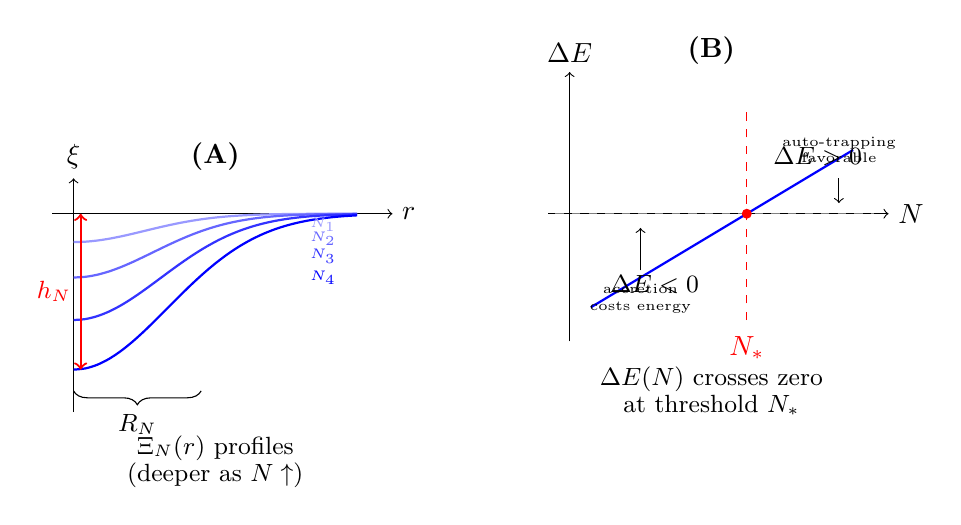
\begin{tikzpicture}[scale=0.9]
% Panel A: Embedding profiles
\begin{scope}[xshift=0cm]
  % Axes
  \draw[->] (-0.3,0) -- (4.5,0) node[right] {$r$};
  \draw[->] (0,-2.8) -- (0,0.5) node[above] {$\xi$};

  % Curves for increasing N
  \draw[thick, blue!40] plot[smooth, domain=0:4] (\x, {-0.4*exp(-(\x)^2/2)});
  \draw[thick, blue!60] plot[smooth, domain=0:4] (\x, {-0.9*exp(-(\x)^2/2.5)});
  \draw[thick, blue!80] plot[smooth, domain=0:4] (\x, {-1.5*exp(-(\x)^2/3)});
  \draw[thick, blue] plot[smooth, domain=0:4] (\x, {-2.2*exp(-(\x)^2/3.5)});

  % Labels
  \node[blue!40, right] at (3.2, -0.15) {\tiny $N_1$};
  \node[blue!60, right] at (3.2, -0.35) {\tiny $N_2$};
  \node[blue!80, right] at (3.2, -0.6) {\tiny $N_3$};
  \node[blue, right] at (3.2, -0.9) {\tiny $N_4$};

  % h_N annotation
  \draw[<->, thick, red] (0.1, 0) -- (0.1, -2.2);
  \node[red, left] at (0.1, -1.1) {\small $h_N$};

  % R_N annotation
  \draw[decorate, decoration={brace, amplitude=5pt, mirror}]
    (0, -2.5) -- (1.8, -2.5);
  \node[below] at (0.9, -2.7) {\small $R_N$};

  % Panel label
  \node at (2, 0.8) {\textbf{(A)}};
  \node[align=center] at (2, -3.5) {\small $\Xi_N(r)$ profiles\\[-0.2em]\small (deeper as $N\uparrow$)};
\end{scope}

% Panel B: Delta E vs N
\begin{scope}[xshift=7cm]
  % Axes
  \draw[->] (-0.3,0) -- (4.5,0) node[right] {$N$};
  \draw[->] (0,-1.8) -- (0,2) node[above] {$\Delta E$};

  % Zero line
  \draw[dashed, gray] (-0.2, 0) -- (4.3, 0);

  % Curve
  \draw[thick, blue] plot[smooth, domain=0.3:4] (\x, {-1.5 + 0.6*\x});

  % N* marker
  \draw[dashed, red] (2.5, -1.5) -- (2.5, 1.5);
  \node[red, below] at (2.5, -1.6) {$N_*$};
  \fill[red] (2.5, 0) circle (2pt);

  % Sign regions
  \node at (1.2, -1) {\small $\Delta E < 0$};
  \node at (3.5, 0.8) {\small $\Delta E > 0$};

  % Annotations
  \draw[->] (1, -0.8) -- (1, -0.2);
  \node[align=center, font=\tiny] at (1, -1.2) {accretion\\costs energy};

  \draw[->] (3.8, 0.5) -- (3.8, 0.15);
  \node[align=center, font=\tiny] at (3.8, 0.9) {auto-trapping\\favorable};

  % Panel label
  \node at (2, 2.3) {\textbf{(B)}};
  \node[align=center] at (2, -2.5) {\small $\Delta E(N)$ crosses zero\\[-0.2em]\small at threshold $N_*$};
\end{scope}
\end{tikzpicture}
\caption{\textbf{(A)} Schematic embedding profiles $\Xi_N(r)$ for increasing
nucleon number $N$; the dimple becomes deeper ($h_N$ increases) and broader
($R_N$ increases) with $N$. \textbf{(B)} The energy gain $\Delta E(N)$
transitions from negative (accretion unfavorable) to positive (auto-trapping)
at the threshold $N_*$ defined by $\Delta E(N_*) = 0$.
\textit{Schematic only; not to scale; definitions/hypothesis; no quantitative claim.}}
\label{fig:autotrap_schematic}
\end{figure}

Figure~\ref{fig:autotrap_schematic} illustrates the core concepts. Panel~(A)
shows how the embedding depth $h_N$ grows with $N$; panel~(B) shows the
threshold behavior of $\Delta E(N)$.

% ============================================================================
\section{What Remains Missing}
% ============================================================================

\begin{statusbox}
The definitions and hypothesis above are \textbf{operational targets} for
a future 5D calculation. The following elements are required to make
quantitative predictions:

\begin{enumerate}
\item \textbf{5D back-reaction computation:} A calculation that maps
$\tau_{\mu\nu}^{(N)} \to \Xi_N(r)$ through the full Einstein equations
in the bulk. This would yield $h_N(N)$ and $E_{\rm env}(r; N)$ explicitly.

\item \textbf{Normalization of $\kappa_5^2$:} The constant $C$ in
$\kappa_5^2 = C \sigma^{-3/4}$ must be fixed (see derivations v3--v5).
Without this, even a complete back-reaction solution cannot predict
$N_*$ numerically.

\item \textbf{Specification of compactification scale $L$:} If $G_N$
is to emerge correctly, the relation $G_N = \kappa_5^2 / (6\pi L)$
requires $L$ (see derivations v1--v2).
\end{enumerate}

\textbf{Conclusion:} BLOCK-003 remains \Open. This document provides
definitions and a hypothesis; it does not constitute a derivation or
a prediction.
\end{statusbox}

% ============================================================================
\section{Summary}
% ============================================================================

\begin{hypothesis}[Auto-Trapping Threshold --- \Open]
\label{hyp:autotrap}
There exists a critical nucleon number $N_*$ such that for $N > N_*$,
the collective brane deformation $\Xi_N(r)$ induces an environmental
energy contribution $E_{\rm env}(r; N)$ making accretion of additional
nucleons energetically favorable ($\Delta E > 0$) without external driving.
\end{hypothesis}

\textbf{What this note does:}
\begin{itemize}
\item Defines $\Xi_N$, $h_N$, $R_N$, $\Delta E(N)$, $N_*$ operationally.
\item Articulates the Israel junction conditions as the bridge between
nucleon binding and bulk geometry.
\item Provides a schematic illustration (Figure~\ref{fig:autotrap_schematic}).
\end{itemize}

\textbf{What this note does not do:}
\begin{itemize}
\item Compute $h_N(N)$ or $E_{\rm env}(r; N)$ from 5D back-reaction.
\item Fix the constant $C$ in $\kappa_5^2$.
\item Predict a numerical value for $N_*$.
\item Close BLOCK-003.
\end{itemize}

\end{document}
